\documentclass{article}
\usepackage{amsmath}
\usepackage{amsfonts}
\usepackage[inline]{enumitem}
\usepackage[a4paper,margin=1in]{geometry}
\usepackage[normalem]{ulem}
\usepackage{graphicx}
\usepackage{tasks}
\settasks{label=(\alph*), label-offset=0.4em, label-width=1.5em}

\usepackage{fancyhdr}
\fancyhf{}
\setlength{\headheight}{36pt}
\renewcommand{\headrulewidth}{0pt}
\thispagestyle{fancy}
\lhead{Calculus Exercise}
\chead{Week 3 (2.5, 2.6, 2.7, 2.8)}
\rhead{\underline{ID:\hspace{7.4em}} \\ \vspace{0.2cm} \uline{Name:\hspace{6em}}}
\cfoot{\thepage}

\begin{document}

\begin{enumerate}
    \item[2.5.30]
        Explain, using Theorems 4, 5, 7, and 9, why the function $B(u) = \sqrt{3u-2} + \sqrt[3]{2u-3}$
        is continuous at every number in its domain. State the domain.

    \vspace{6cm}

    \item[2.5.36]
        Use continuity to evaluate the limit $\displaystyle \lim_{\theta \to \pi/2} \sin\left(\tan\left(\cos{\theta}\right)\right)$

    \vspace{6cm}

    \item[2.5.44]
        Find the numbers at which $f$ is discontinuous.
        At which of these numbers is $f$ continuous from the right, from the left, or neither? Sketch the graph of $f$
        \begin{equation*}
            f(x) =
            \begin{cases}
                2^x & \text{if} \ x \leq 1 \\
                3 - x & \text{if} \ 1 < x \leq 4 \\
                \sqrt{x} & \text{if} \ x > 4
            \end{cases}
        \end{equation*}

    \vspace{6cm}

    \item[2.5.48]
        Find the values of $a$ and $b$ that make $f$ continuous everywhere.
        \begin{equation*}
            f(x) =
            \begin{cases}
                \frac{x^2 - 4}{x - 2} & \text{if} \ x < 2 \\
                ax^2 - bx + 3 & \text{if} \ 2 \leq x < 3 \\
                2x - a + b & \text{if} \ x \geq 3
            \end{cases}
        \end{equation*}

    \vspace{6cm}

    \item[2.5.58]
        Use the Intermediate Value Theorem to show that there is a solution of
        the given equation $\sin{x}=x^2-x$ in the interval $(1,2)$.

    \vspace{6cm}

    \item[2.6.30]
        Find the limit of $\displaystyle \lim_{x \to -\infty} \left( \sqrt{4x^2+3x} + 2x\right)$ or show that it does not exist.

    \newpage

    \item[2.6.48]
        Find the horizontal and vertical asymptotes of the curve $y=\dfrac{2x^2+1}{3x^2+2x-1}$.
        You may want to use a graphing calculator (or computer) to check your work by
        graphing the curve and estimating the asymptotes.

    \vspace{8cm}

    \item[2.6.58]
        Find a formula for a function that has vertical asymptotes $x = 1$ and $x = 3$ and horizontal asymptote $y = 1$.

    \vspace{6cm}

    \item[2.7.34]
        If the tangent line to $y = f(x)$ at $(4, 3)$ passes through the point $(0, 2)$, find $f(4)$ and $f^{\prime}(4)$.

    \newpage

    \item[2.7.42]
        Sketch the graph of a function $f$ where the domain is $(-2, 2)$, $f^{\prime}(0)=-2$,
        $\displaystyle \lim_{x \to 2^-}f(x)=\infty$, $f$ is continuous at all numbers in its domain except $\pm 1$,
        and $f$ is odd.

    \vspace{6cm}

    \item[2.7.58]
        Determine whether $f^{\prime}(0)$ exists, where
        \begin{equation*}
            f(x) =
            \begin{cases}
                x^2 \sin{\frac{1}{x}} & \text{if} \ x \neq 0\\
                0 & \text{if} \ x=0
            \end{cases}.
        \end{equation*}

    \vspace{6cm}

    \item[2.8.40]
        Suppose $N$ is the number of people in the United States who travel by car to another state
        for a vacation in a year when the average price of gasoline is $p$ dollars per gallon.
        Do you expect $\frac{dN}{dp}$ to be positive or negative? Explain.

    \newpage

    \item[2.8.52]
        The figure shows the graphs of four functions.
        One is the position function of a car, one is the velocity of the car, one is its acceleration, and one is its jerk.
        Identify each curve, and explain your choices.

        \begin{center}
            \includegraphics[width=7cm]{./png/2.8.52.png}
        \end{center}

    \vspace{6cm}

    \item[2.8.63]
        Recall that a function $f$ is called \textit{even} if $f(-x)=f(x)$ for all $x$ in its domain
        and \textit{odd} \\ if $f(-x)=-f(x)$ for all such $x$. Prove each of the following

        \begin{enumerate}
            \item The derivative of an even function is an odd function.
            \item The derivative of an odd function is an even function.
        \end{enumerate}


\end{enumerate}
\end{document}
